\scanpage{245}

% top, slightly right of centre
\mspage{99}

% top half, six-node implication schema
{\scriptsize\diagram{\begin{tikzcd}[ampersand replacement=\&,row sep=large,column sep=small,scale=.80,transform shape]
\&{\substack{X\ \text{\uline{cofiltrante}}\\
(\mathrm{PS}^{*}1'+\mathrm{PS}^{*}2\\ \deleted{\Leftrightarrow}\ \unsure{\mathrm{PS}^{*}1|{\mathrm{PS}}}\,1+\mathrm{PS}^{*}2+\text{0-conn})}}
\arrow[dl,Rightarrow]\arrow[d,Rightarrow,"\substack{\deleted{\unsure{\Rightarrow|\mathrm{PS}}}\mathrm{PS}^{*}1'\\(\Rightarrow\text{0-conn})}"']
\arrow[dr,Rightarrow,"\substack{\mathrm{PS}^{*}1\\(\text{les }{}_{a\backslash}X\text{ satisfont}\\ \mathrm{PS}^{*}1')}"']
\&\\
{\substack{\text{\textcircled{\(\triangle\)}}\quad X\text{ tot 0-conn}\\(X^\circ\to X^\circ\times X^\circ\ \text{cofinal})}}\arrow[d,Rightarrow]
\&{\substack{X\ \text{\uline{\unsure{pscofiltrante|pseudofiltrante|pscofiltrant}}}\\\text{0-connexe}\\(\mathrm{PS}^{*}1+\text{0-conn.})\\(\text{manque }\mathrm{PS}^{*}2)\\\text{\textcircled{\(B_G\)}}\\G\ne\{1\}}}\arrow[dl,Rightarrow]\arrow[dr,Rightarrow]
\&{\substack{\text{\textcircled{\(\unsure{\varepsilon|e}=\substack{\bullet\\[-.65ex]\bullet}\)}}\\
\underbrace{(\text{\unsure{comp.|compos.} conn. filtrantes})}\\X\ \text{\uline{loc. cofiltrante}}\\
(\mathrm{PS}^{*}1+\mathrm{PS}^{*}2)}}\arrow[d,Rightarrow]\\
{\substack{X\text{ irréductible}\\(\mathrm{PS}^{*}1')\\
\text{\textcircled{\(\bullet\rightrightarrows\bullet\)}}}}
\&\&{\substack{\underbrace{(\text{comp. conn. ps. filtrantes})}\\
X\ \text{\uline{pseudo-cofiltrante}}\\ \text{ou encore \uline{loc. irréductible}}\\
(\mathrm{PS}^{*}1.)\\ \text{\textcircled{\(B_G\amalg e\)}}\\G\ne\{1\}}}
\end{tikzcd}}}

% centre above second schema
et dualement on a $\downarrow$

% lower half, six-node dual schema
{\small\diagram{\begin{tikzcd}[ampersand replacement=\&,row sep=large,column sep=small,scale=.80,transform shape]
\&{X\ \text{\deleted{co}filtrante}}\arrow[dl,Rightarrow]\arrow[d,Rightarrow]\arrow[dr,Rightarrow]\&\\
{X^\circ\text{ tot. 0-connexe}}\arrow[d,Rightarrow]\&
{\substack{X\text{ ps-filtrante}\\\text{0-conn.}}}\arrow[dl,Rightarrow]\arrow[dr,Rightarrow]\&
{X\text{ loc. filtrante}}\arrow[d,Rightarrow]\\
{X\text{ coirréductible}}\&\&{X\text{ ps-filtrante}}
\end{tikzcd}}}

% below dual schema, left
donc on a une terminologie \unsure{décente|directe} sauf pour ``$X^\circ$ tot. 0-connexe'' -- je n'ose dire ``$X$ \unsure{tot.|dét.} co-connexe''!!

% inverted printed letterhead, left column when upright
% letterhead
\deleted{MINISTERE DE L'EDUCATION NATIONALE\\
ACADEMIE D'AIX-MARSEILLE\\
\rule{2em}{.3pt}\\
Inspection Académique\\
de Vaucluse\\
\rule{2em}{.3pt}\\
Tél. : 90 82 99 76\\
Référence : Secrétariat n\textsuperscript{o}}

% inverted printed letterhead, right column when upright
% letterhead
\deleted{AVIGNON, le\\
L'Inspecteur d'académie,\\
directeur des services départementaux\\
de l'Education Nationale de Vaucluse,\\
à M}

% bottom left over the letterhead, two outlines joined by diagonals
\handwritten{\figure{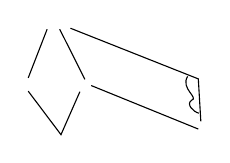
\begin{tikzpicture}[x=.8cm,y=.65cm]
\draw (0,1.15)--(.3,2.1) (.5,2.1)--(.9,1.12) (1,1)--(2.7,.15) (.67,2.12)--(2.7,1.13)--(2.74,.3) (0,.89)--(.52,.04)--(.82,.88);
\draw (2.53,1.18) .. controls (2.41,.94) and (2.72,.76) .. (2.59,.71) .. controls (2.5,.63) and (2.63,.48) .. (2.71,.46);
\end{tikzpicture}}}

% bottom centre-right, three uprights connected by sloping lines
\handwritten{\figure{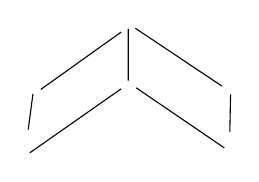
\begin{tikzpicture}[x=1cm,y=.7cm]
\draw (0,.45)--(.06,1.1) (.16,1.18)--(1.18,2.22) (1.27,2.28)--(1.27,1.34) (1.36,2.29)--(2.46,1.24) (2.57,1.09)--(2.56,.41) (1.37,1.21)--(2.49,.12) (1.18,1.19)--(.02,.03);
\end{tikzpicture}}}

% archive sheet number: 245
